\documentclass{beamer}

\usepackage{tikz}
\usepackage{tkz-berge} 
\usepackage{algorithm,algorithmic}
\mode<presentation>

{
  \usetheme{Warsaw}

 \setbeamertemplate{footline}{}
\setbeamercovered{transparent}
\usepackage{color}
\title{A programming approach to vertex coloring by kernelization}
\author{{Mehri Bagherihamaneh}\\[1cm]{\small {Advisor: Prof. Dr. Arie M.C.A. Koster}}\\[.5cm]{\small {Lehr-und Forschungsgebiet Diskrete Optimierung}}\\ {\small {Rheinisch-Westfaelische Technische Hochschule Aachen}}}

{\small \date{{Aachen, }\today}}


\begin{document}

\begin{frame}
  \titlepage
\end{frame}


\begin{frame}{What this thesis is about?}
\begin{itemize}

\item Graph vertex coloring

\item Using kernelization to solve vertex coloring with reduction of size of the  graph
\item Demonstrate kernelization in some sample graphs in practice
\item "improved DSATUR-based Branch and Bound" algorithm
\item Python is used as programming language

\end{itemize}
\end{frame}

\begin{frame}{Introduction}


\begin{enumerate}
\item Some definitions
\item Special kernelization for vertex coloring

\item Min vertex cover
\item An example

\item An exact algorithm for vertex coloring

\item Computational experiments
\item conclusion
\end{enumerate}
\end{frame}



\begin{frame}{Definitions}


\begin{definition}
A vertex coloring is an assignment of labels or colors to each
vertex of a graph such that no edge connects two vertices with the same color.

The chromatic number of a graph is the smallest number of colors needed for
vertex coloring and denoted by $\chi(G)$. 

A vertex coloring of a graph with $k$ or fewer colors is known as a $k$-coloring. A proper $k$-coloring is an assignment of $k$ colors to the vertices of a graph so that no two adjacent vertices have the same color. 

A proper $k$-coloring of a graph $G$ can be shown as a function $f: V(G) \to \{1, 2, 3, . . . , k\}$ such that adjacent vertices get different colors, namely in a proper coloring, for all edges $\{u, v\}$ we have $f(u) \not= f(v)$.
\end{definition}
\end{frame}


\begin{frame}{Definitions}
\begin{example}
The petersen graph is $3$-colorable:

\begin{center}
\begin{tikzpicture}[rotate=90]
  \GraphInit[vstyle=Hasse]
  \SetVertexNoLabel \SetUpVertex[MinSize=2pt] \grPetersen[RA=2,RB=1]
  \SetUpVertex[inner sep=1pt,MinSize=2pt]
  \AddVertexColor{red}{a0,b1,b2,a3}
  \AddVertexColor{green}{a1,b0,a4}
  \AddVertexColor{blue}{b4,b3,a2}
\end{tikzpicture}
\end{center}
\end{example}
\end{frame}

\begin{frame}{Propositional logic}
\begin{definition}
A propositional logic formula is constructed by some variables using operators AND ("$\land$"), OR ("$\lor$"), NOT ("$\lnot$") and parentheses. 

A clause is an expression constructed from a finite  disjunction or conjunction of literals.
\end{definition}



\begin{definition}
A boolean formula is satisfiable if it can be TRUE by assigning logical values to its variables. 
\end{definition}
\end{frame}
\begin{frame}{Propositional logic}


\begin{example}

\item $x_1 \land (x_2 \lor\lnot x_1)$, where $(x_2 \lor\lnot x_1)$ is a clause.

\end{example}
\begin{example}
 $\varphi = d\lor (a\land b\land (c\lor d \land\lnot a))$

\begin{table}[H]
\begin{center}
\begin{tabular}{c|c|c|c|c}
$a$ & $b$ & $c$ & $d$ & $\varphi$\\
\hline
F & F & F & T & T\\ 
&&&&\\
&&&&\\
\end{tabular}
\end{center}
\end{table}
\end{example}

\begin{example}
Unsatisfiable formula:

\begin{center}
$\theta = X \land \lnot X$
\end{center}
\end{example}

\end{frame}

\begin{frame}{Propositional logic}
\begin{definition}
A boolean formula is in conjunctive normal form (CNF) if it is a conjunction of one or more disjunctions of variables.
\end{definition}

\begin{example}
\item $\lnot x \land (y \lor z)$
\end{example}

\begin{definition}
For a given CNF formula $\varphi$, the boolean satisfiability problem (SAT) is a decision problem which asks whether the formula $\varphi$ is satisfiable. The $3$-SAT problem is a SAT problem with at most $3$ variables in each clause. 
\end{definition}

\begin{theorem}
The $3$-SAT problem is $NP$-complete.
\end{theorem}
\end{frame}


\begin{frame}{Complexity}
\begin{definition}
For an instance $I$ from instance set $\mathcal{I}$, a decision problem $\Pi$ is a YES-NO question which asks if
there is at least one solution for the problem $\Pi$ in $I$.
\end{definition}
\begin{example}
$k$-COLORING is a decision problem, which asks if we can color a graph $G$ with $k\in\mathbb{N}$ or fewer colors. For $k \geq 3$ in general graphs, $k$-COLORING is $NP$-complete.
\end{example}
\end{frame}


\begin{frame}{Complexity}
\begin{itemize}
\item class $P$ (PTIME)

\color{green} Example: \color{black} the problem of determining if a number is prime.

\item $NP$ (non-deterministic polynomial) $P\subset NP$.

\item $NP$-hard class 

\color{green} Example: \color{black} traveling salesman problem.

If $P \not= NP$, $NP$-hard problems cannot be solved in polynomial time. 

\item $NP$-complete class:  $L$ is $NP$-complete if:
\begin{enumerate}
\item $L$ is $NP$-hard.

\item $L$ is in $NP$.
\end{enumerate}
\end{itemize}
\end{frame}


\begin{frame}{Is $P = NP$ or $P \not= NP$?}

%\vspace{2cm}
\newcommand{\boundellipse}[3]% center, xdim, ydim
{(#1) ellipse (#2 and #3)
}

\begin{figure}[!ht]
\centering


\begin{tikzpicture}
\draw (0,0) circle (1.5cm);
\draw \boundellipse{0,-0.75}{1.1}{0.75};
\draw (-1.5,3) .. controls (-1,0) and (1,0) .. (1.5,3);
\node at (0,2) {\tiny $NP$-Hard};
\node at (0,1.2) {\tiny $NP$-Complete};
\node at (-1,0) {\tiny $NP$};
\node at (0,-0.75) {\tiny $P$};
\node at (0,-2) {\tiny $P \not= NP$};
\node at (4,1) [label={[rotate=90]{\tiny complexity}}];
\draw[->] (4,-2) -- (4,4);
\draw (8,0) circle (1.5cm);

\draw (6.5,2) .. controls (5.40,-2.7) and (10.6,-2.7) .. (9.5,2);
\node at (8,2) {\tiny $NP$-Hard};
\node at (8,0) {\tiny $NP$-Complete = $P$ = $NP$};

\node at (8,-2) {\tiny $P = NP$};
\end{tikzpicture}
\caption{\tiny Euler diagram for $P$, $NP$, $NP$-hard and $NP$-complete set of problems}
\end{figure}
\end{frame}

\begin{frame}{Parameterized Complexity}

If we assume $P \not = NP$, for small parameter  $k$ (but large instance), we can use efficient exact algorithms. 

\begin{definition}
A parameterized problem is a pair $(\Pi, \kappa)$ in which $\Pi$ is a
decision problem with instance set $\mathcal{I}$ and $\kappa : \mathcal{I} \to \mathbb{N}$, which is a polynomial
time computable function, called parameter.
\end{definition}

\begin{example}
Parameterized-vertex cover, denoted $k$-VERTEX COVER:

Input : graph $G = (V, E)$ and a number $k \in \mathbb{N}$

parameter : $k$

problem : Is there any vertex cover set in $G$ with maximum size of $k$?
\end{example}

\end{frame}

\begin{frame}{Kernelization}

\begin{definition}
Let $(\Pi, \kappa)$ be a parameterized problem, $I\in\mathcal{I}$ an instance and $\kappa: \mathcal{I} \to \mathbb{N}$ a parameterization for $\Pi$:

A polynomial time computable function $f : \mathcal{I} \times \mathbb{N} \to \mathcal{I} \times \mathbb{N}$ is called a
kernelization for $(\Pi, \kappa)$ , if $f(I, \kappa(I)) = (I', \kappa(I'))$ such that it satisfies these 3 properties:

\begin{enumerate}[(i)]
\item For each $I \in \mathcal{I}$, $(I, \kappa(I))$ is a "YES"-instance of $\Pi$ iff $(I', \kappa(I'))$ is a "YES"-instance of $\Pi$.

\item There is a function $f': \mathbb{N} \to \mathbb{N}$, such that $|I'| \leq f'(\kappa(I))$

\item $\kappa(I')\leq \kappa(I)$.
\end{enumerate}

$I'$ is kernel of $(\Pi, \kappa)$ and $f'(\kappa(I))$ is called the size of the kernel.

\end{definition}

\end{frame}

\begin{frame}{Kernelization}
\begin{example}
Kernelization of the vertex cover problem:

Input: Graph $G$ and a positive integer $k$ 

Output: A vertex cover set with at most size $k$


\begin{itemize}
\item If $v$ is an isolated vertex of $G$, we remove $v$. The new instance is $(G - v , k)$.


\item If $G$ contains a vertex $v$ of degree greater than $k$, remove $v$ from the graph and decrease $k$ by one. The new instance is $(G - v , k - 1)$.

\item If neither of the previous two rules can be applied anymore,
\begin{itemize}
\item If the graph still has more than $k^2$ edges, the problem has no solution.

\item If the graph has at most $k^2$ edges, it has at most $2 k^2$ vertices, hence the size of the kernel is at most $2 k^2$.
\end{itemize}

  
\end{itemize}



The problem can be solved in time $\mathcal{O}(2^{2k^2} + |V| + |E|)$.
\end{example}
\end{frame}


\begin{frame}{Kernelization of the Vertex Coloring}
A kernelization on $3$-coloring using vertex cover:

\begin{enumerate}
\item Compute $2$-approximate vertex cover $X$

\item $\forall S\subseteq X$ of size $3$
\begin{itemize}
\item Mark a common neighbor of $S$
\end{itemize}
\item Delete all unmarked $v \not\in X$

\item Output resulting $G'$ on $n'$ vertices:

\begin{center}
$n' \leq |X| + |X|^3 \leq 2k + (2k)^3$
\end{center}
\end{enumerate}

$G$ is $3$-colorable iff $G'$ is $3$-colorable. Run time for the algorithm is $\mathcal{O}(min|X|^3)$.


\begin{theorem}{\label{main theorem}}
$G$ is $q$-colorable iff $G'$ is $q$-colorable. Run time for the algorithm
is $\mathcal{O}(min|X|^q)$.
\end{theorem}
\end{frame}

\begin{frame}{Revision of the algorithm}

\begin{algorithm}[H]
\begin{algorithmic}[1]
\SetAlgoLined
\DontPrintSemicolon
  \caption{Kernelization of vertex coloring by using vertex cover}

\STATE Find exact minimum vertex cover\\

\STATE Iterate all vertices outside of vertex cover\\

\STATE If the vertex has $3$ distinct neighbors in vertex cover and it wasn't
visited yet, then mark it\\

\STATE Delete all unmarked vertices outside of vertex cover\\
\end{algorithmic}
\end{algorithm}
\end{frame}


\begin{frame}{Minimum Vertex Cover}

\begin{align*}
&minimize \; \;\; \; \sum_{v\in V}X_v \\
&subject\; to \;\;\; \; X_u + X_v  \geq 1 , \qquad \\
&\qquad 	\qquad\qquad\qquad	 \forall \{u,v\} \in E\\
&and	\qquad\qquad	 \forall v, X_v\in \{0,1\}
\end{align*}
\end{frame}


\begin{frame}{Minimum Vertex Cover}
We can restrict this ILP to maximal cliques inequality:


\begin{align*}
&minimize \; \;\; \; \sum_{v\in V}X_v\\
&subject\; to \;\;\; \; X_u + X_v  \geq 1 ,\\
&\qquad 	\qquad\qquad\qquad	 \forall \{u,v\} \in E\\
&and	\qquad\quad\;\; \sum_{v\in K_n}x_v \geq n - 1\\
& \qquad\qquad \qquad\qquad for\; every\; maximal\; clique\; K_n\; in\; the\; graph\\
&and	\qquad\qquad	 \forall v, X_v\in \{0,1\}
\end{align*}
\end{frame}


\begin{frame}{Minimum Vertex Cover}
Every edge is also a clique:


\begin{align*}
&minimize \; \;\; \; \sum_{v\in V}X_v\\
&subject\; to \;\;\; \; \sum_{v\in K_n}x_v \geq n - 1\\
& \qquad\qquad \qquad\qquad for\; every\; maximal\; clique\; K_n\; in\; the\; graph\\
&and	\qquad\qquad	 \forall v, X_v\in \{0,1\}
\end{align*}



\end{frame}

\begin{frame}{Maximal Clique}


\begin{algorithm}[H]
\begin{algorithmic}[1]

\STATE BronKerbosch({$R, P, X$})\\

        \IF{$P$ and $X$ are both empty}{
        
		  	 report $R$ as a maximal clique\\	
		 }\ENDIF
		\FOR{vertex $v$ in $P$}{
		
			   BronKerbosch$(R \cup \{v\}, P \cap N(v), X \cap N(v))$
			   
			    $P := P\setminus \{v\}$
			    
			   	   $X := X\cup \{v\}$\\
		}\ENDFOR

\end{algorithmic}
\caption{Bron-Kerbosch}
\end{algorithm}

\end{frame}

\begin{frame}{An Example}
This graph has $11$ vertices and $20$ edges and is known to be $4$-colorable:

\vspace{0.5cm}
\begin{center}
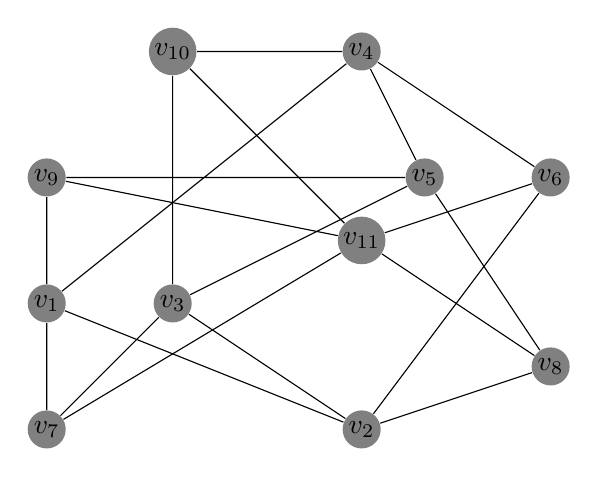
\begin{tikzpicture}[scale=0.8]
\node[circle,fill=gray,inner sep=1pt,minimum size=1mm] (v1) at (0,0) {$v_1$};
\node[circle,fill=gray,inner sep=1pt,minimum size=1mm] (v2) at (5,-2) {$v_2$};
\node[circle,fill=gray,inner sep=1pt,minimum size=1mm] (v3) at (2,0) {$v_3$};
\node[circle,fill=gray,inner sep=1pt,minimum size=1mm] (v4) at (5,4) {$v_4$};
\node[circle,fill=gray,inner sep=1pt,minimum size=1mm] (v5) at (6,2) {$v_5$};
\node[circle,fill=gray,inner sep=1pt,minimum size=1mm] (v6) at (8,2) {$v_6$};
\node[circle,fill=gray,inner sep=1pt,minimum size=1mm] (v7) at (0,-2) {$v_7$};
\node[circle,fill=gray,inner sep=1pt,minimum size=1mm] (v8) at (8,-1) {$v_8$};
\node[circle,fill=gray,inner sep=1pt,minimum size=1mm] (v9) at (0,2) {$v_9$};
\node[circle,fill=gray,inner sep=1pt,minimum size=1mm] (v10) at (2,4) {$v_{10}$};
\node[circle,fill=gray,inner sep=1pt,minimum size=1mm] (v11) at (5,1) {$v_{11}$};


\draw (v4)--(v1)--(v2)--(v3)--(v5)--(v9)--(v1);
\draw (v1)--(v7)--(v3)--(v10)--(v4)--(v6)--(v2)--(v8)--(v11);
\draw (v7)--(v11)--(v10);
\draw (v9)--(v11)--(v6);
\draw (v4)--(v5)--(v8);
\end{tikzpicture}
\end{center}


\end{frame}

\end{document}
}